\ifdefined\MAINDOC\else
\documentclass[10pt, a4paper, fleqn]{article}
\usepackage{base}

\begin{document}
    \title{Skript Mathe 2}
    \date{30. Mai 2018}
    \maketitle
\fi
    \begin{enumerate}[a), start=9]
        \item[]
        \begin{enumerate}[1.]
            \item Dabei wird der Winkel $\varphi$ meistens im Bogenmaß
            angegeben, d.h. $\varphi \in [0, 2 \pi]$. 
            
            Einige wichtige Werte:

            {\def\arraystretch{1.5}             
            \begin{tabular}{|r|c|c|c|c|c|c|}
                \hline
                Gradmaß: & $0^\circ$ & $30^\circ$ & $45^\circ$ & $60^\circ$ & $90^\circ$ & $180^\circ$ \\
                \hline
                Bogenmaß: & $0$ & $\frac{\pi}{6}$ & $\frac{\pi}{4}$ & $\frac{\pi}{3}$ & $\frac{\pi}{2}$ & $\pi$ \\
                \hline
                $\sin$: & $0$ & $\frac{1}{2}$ & $\frac{1}{\sqrt{2}}$ & $\frac{\sqrt{3}}{2}$ & $1$ & $0$ \\
                \hline
                $\cos$: & $1$ & $\frac{\sqrt{3}}{2}$ & $\frac{1}{\sqrt{2}}$ & $\frac{1}{2}$ & $0$ & $-1$ \\
                \hline
            \end{tabular}}

            Daraus können weitere Werte mit Hilfe des Einheitskreises abgeleitet werden:
            
            \begin{minipage}{0.6\textwidth}
                \begin{tikzpicture}
                    \begin{axis}[
                        clip = false,
                        width = \textwidth,
                        height = \textwidth,
                        xmin = -1.2, xmax = 1.2,
                        ymin = -1.2, ymax = 1.2,
                        xtick distance = 1,
                        ytick distance = 1,
                        axis x line = center,
                        axis y line = center,
                        axis line style = {->}
                    ]
                    \coordinate (A) at (0, 0);
                    \coordinate (B) at ({cos(60)}, {sin(60)});
                    \coordinate (C) at ({cos(60)}, 0);
                    \coordinate (D) at ({cos(120)}, {sin(120)});
                    \coordinate (E) at ({cos(120)}, 0);
        
                    \addplot [domain = 0:360, samples = 100] ({cos(x)}, {sin(x))});
                    \draw (A) -- (B) -- (C) -- (A);
                    \draw (A) -- (D) -- (E) -- (A);
                    
                    \draw pic["$\frac{\pi}{3}$", angle radius = 18pt, draw = black] {angle = C--A--B};
                    \draw pic[angle radius = 23pt, draw = black] {angle = C--A--D};
                    \draw [->] (-0.8, 1) node[left] {$\frac{2\pi}{3}$} -- (-0.05, 0.2);

                    % Braces
                    \draw[decorate, decoration = {brace, mirror, amplitude = 5pt, raise = 2pt}] 
                        (A) -- (C) node[midway, yshift = -15pt] {$\frac{1}{2}$};
                    \draw[decorate, decoration = {brace, mirror, amplitude = 5pt, raise = 2pt}] 
                        (E) -- (A) node[midway, yshift = -15pt] {$-\frac{1}{2}$};
                    \draw[decorate, decoration = {brace, mirror, amplitude = 5pt, raise = 2pt}]
                        (C) -- (B) node[midway, right, xshift = 5pt] {$\frac{\sqrt{3}}{3}$};
                    
                    \end{axis}
                \end{tikzpicture}
            \end{minipage}
            \begin{minipage}{0.4\textwidth}
                \[\begin{aligned}
                    &\cos\qt{\frac{2\pi}{3}} = -\frac{1}{2} = -\cos\qt{\frac{\pi}{3}} \\
                    &\sin\qt{\frac{2\pi}{3}} = \frac{\sqrt{3}}{2} = -\sin\qt{\frac{\pi}{3}} \\
                \end{aligned}\]
            \end{minipage}
            \item $\sin$ und $\cos$ sind nicht bijektiv. Jedoch ist
            $\sin [-\frac{\pi}{2}, \frac{\pi}{2}] \to [-1, 1]$ und $\cos [0, \pi] \to [-1, 1]$ bijektiv.
            Die Umkehrfunktionen sind:

            \begin{tabular}{rl}
                $\arcsin$: & $[-1, 1] \to [-\frac{\pi}{2}, \frac{\pi}{2}]$ \\
                $\arccos$: & $[-1, 1] \to [0, \pi]$
            \end{tabular}

            Entsprechend erhält man:

            \begin{tabular}{rl}
                $\arctan$: & $\IR \to (-\frac{\pi}{2}, \frac{\pi}{2})$ \\
                $\arccotan$: & $\IR \to (0, \pi)$
            \end{tabular}

            \item
            \begin{itemize}
                \item Es ist $\sin(x + \frac{\pi}{2}) = \cos(x) \quad \forall x \in \IR$
                \item $\sin, \cos$ sind $2\pi$-periodisch, d.h. \\
                $\sin(x + 2 \pi) = \sin(x), \cos(x + 2 \pi) = \cos(x)$
                \item $\tan, \cotan$ sind $\pi$-periodisch
            \end{itemize}

            \item Symmetrien
            \[\begin{aligned}
                \cos(x) &= \cos(-x) & \forall x \in \IR \\
                \sin(x) &= -\sin(-x) & \forall x \in \IR \\
                \tan(x) &= -\tan(-x) &\forall x \in \IR \\
                \cotan(x) &= -\cotan(-x) & \forall x \in \IR
            \end{aligned}\]

            \item Rechenregeln
            \begin{enumerate}[a)]
                \item $\sin x + \cos x = 1 \quad \forall x \in \IR$
                \item Additionstheoreme
                \begin{itemize}
                    \item $\sin(x+y) = \sin(x) \cdot \cos(y) + \cos(x) \cdot \sin(y)$
                    \item $\cos(x+y) = \cos(x) \cdot \cos(y) - \sin(x) \cdot \sin(y)$
                \end{itemize}
            \end{enumerate}
        \end{enumerate}
    \end{enumerate}

    \section{Grenzwerte von Funktionen und Stetigkeit}
    \subsection{Definition: Grundbegriffe und Beispiele}

    Sei $M \subseteq \IR$.
    \begin{enumerate}[a)]
        \item $X_0 \in \IR$ heißt Häufungspunkt von $M$ \\
         $:\eqv$ Es gibt eie Folge $(X_n)$ in
        $M \setminus \{X_0\}$ mit $X_n \mapsto X_0$
        
        \item $X_0 \in M$ heißt isolierter Punkt von $M$ \\
        $:\eqv X_0$ ist kein Häufungspunkt von M
    \end{enumerate}

    \subsection{Beispiele}
    \begin{enumerate}[a)]
        \item $M = (0, 1) \cup \{2\} \cup (3, 4)$
        \begin{itemize}
            \item Menge der Häufungspunkte von $M$: \\
            $H = [0,1] \cup [3,4]$
            denn z.B für $X_0 = \frac{1}{2}$ hat die Folge
            $(\frac{1}{2} - \frac{1}{n})_{n \geq 3}$ den Limes
            $X_0$ und liegt in $M \setminus \{X_0\}$.

            Auf analoge Weise können für jedes andere $X_0 \in M$ \\
            Folgen in $M \setminus \{X_0\}$ konstruiert werden.

            \item Einziger isolierter Punkt in $M$ ist $2$, denn es gibt in \\ 
            $M \setminus \{2\} = (0,1) \cup (3,4)$ keine Folge
            mit Grenzwert $2$.
        \end{itemize}
        \item $M = \{\frac{1}{n} \ | \ n \in \IN\}$
        \begin{itemize}
            \item Menge der HP von $M$: $\{0\}$
            \item Menge der isolierten Punkte: $M$
        \end{itemize}
    \end{enumerate}

    \subsection{Bemerkung}
    Ein isolierter Punkt $X_0$ von $M$ liegt vor, wenn es ein $\epsilon > 0$ gibt,
    so dass \\ $|X - X_0| \geq \epsilon \quad \forall x \in M \setminus \{X_0\}$,
    z.B ist in 5.2a $|X - 2| \geq 1 \quad \forall x \in M \setminus \{2\}$

    \subsection{Definition Grenzwert I}
    Sei $f: D \to \IR$ reelle Funktion und $a \in \IR$.
    Ist $X_0$ ein Häufungspunkt von $D$, so sagt man $f$ hat in $X_0$ den Grenzwert
    $a$, oder $f(x)$ konvergiert gegen $a$ für $x \to a :\eqv \lim\limits_{n \to \infty} f(X_n) = a$,
    für jede beliebige Folge $(X_n)$ in $D \setminus \{X_0\}$ mit $X_n \to X_0$.

    Schreibweise: $\lim\limits_{x \to X_0} f(x) = a$ oder
    $f(x) \to a$ für $x \to X_0$

    \subsection{Beispiele}
    \begin{enumerate}[a)]
        \item $f: \IR \to \IR, x \mapsto x^2, X_0 = 1$

        Für $(X_n)$ in $\IR \setminus \{1\}$ mit $X_n \to 1$ ist
        $f(X_n) = {X_n}^2 \xrightarrow[n \to \infty]{} 1$ (1.13/3)

        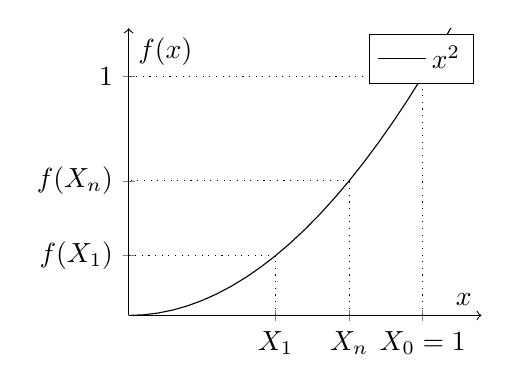
\begin{tikzpicture}[
                declare function = {f(\x) = \x^2;}
            ]
            \begin{axis}[
                width = 0.5\textwidth,
                xlabel = {$x$},
                ylabel = {$f(x)$},
                xmin = 0, ymin = 0,
                xmax = 1.2, ymax = 1.2,
                axis x line = center,
                axis y line = center,
                axis line style = {->},
                xtick = {0.5, 0.75, 1},
                xticklabels = {$X_1$, $X_n$, $X_0 = 1$},
                ytick = {0.25, 0.5625, 1},
                yticklabels = {$f(X_1)$, $f(X_n)$, $1$},
                domain = 0:1.2
            ]
            \draw[dotted] (0.5, 0) -- (0.5, {f(0.5)}) -- (0, {f(0.5)});
            \draw[dotted] (0.75, 0) -- (0.75, {f(0.75)}) -- (0, {f(0.75)});
            \draw[dotted] (1, 0) -- (1, 1) -- (0, 1);

            \addplot[color = black] {f(x)};
            \legend{$x^2$}
            \end{axis}
        \end{tikzpicture}

        \item Es muss für jede Folge $(X_n)$ in $D \setminus \{X_0\}$ mit $X_n \to X_0$ gelten:
        $f(X_n) \to a$

        Gegenbeispiel: $f: \IR \to \IR \quad f(x) = \begin{cases}
            -1 & x < 0 \\
            +1 & x > 0
        \end{cases}$

        \begin{tikzpicture}[
            declare function = {f(\x) = \x^2;}
        ]
        \begin{axis}[
            width = 0.6\textwidth,
            height = 0.3\textwidth,
            xlabel = {$x$},
            ymin = -1.2, ymax = 1.2,
            xmin = -1, xmax = 1,
            xtick = \empty,
            axis x line = center,
            axis y line = center,
            axis line style = {->},
            samples at = {-1, -0.001, 0, 0.001, 1}
        ]
        \addplot[color = black] {sign(x)};  
        \end{axis}
    \end{tikzpicture}

    Grenzwert in $X_0 = 0$ existiert nicht, denn \\
    $f(-\frac{1}{n}) = -1 \xrightarrow[n \to \infty]{} -1$ und \\
    $f(\frac{1}{n}) = 1 \xrightarrow[n \to \infty]{} 1$, obwohl 
    $\frac{-1}{n} \to X_0$ und $\frac{1}{n} \to X_0$
    \end{enumerate}

    \subsection{$\epsilon$--$\varphi$--Kriterium}
    Sei $f: D \to \IR$ reelle Funktion, $X_0$ HP in $D$,
    $a \in \IR$. Dann:
    \[\begin{aligned}
        \lim_{x \to X_0} f(x) = a \eqv \forall \epsilon > 0 \ \forall x \in D \setminus \{X_0\}: \\
        \underbrace{|x-X_0| < \delta \imp |f(x) - a| < \epsilon}_{(*)}
    \end{aligned}\]

\iffalse %TODO Figure out what the graph for this is
    \textbf{Anschaulich:}

    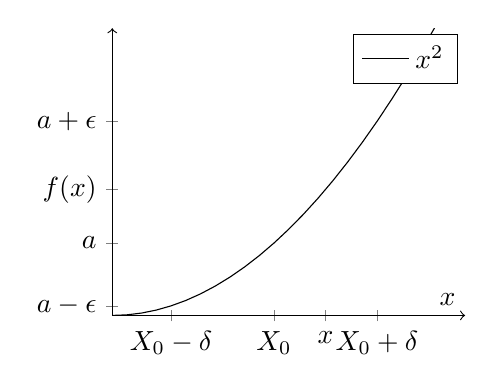
\begin{tikzpicture}[
        declare function = {f(\x) = \x^2;}
    ]
        \begin{axis}[
            width = 0.5\textwidth,
            xlabel = {$x$},
            xmin = 0, ymin = 0,
            xmax = 1.2, ymax = 1.2,
            axis x line = center,
            axis y line = center,
            axis line style = {->},
            xtick = {0.2, 0.55, 0.725, 0.9},
            xticklabels = {$X_0 - \delta$, $X_0$, $x$, $X_0 + \delta$},
            ytick = {0.04, 0.3025, 0.525625, 0.81},
            yticklabels = {$a - \epsilon$, $a$, $f(x)$, $a + \epsilon$},
            domain = 0:1.2
        ]
        \addplot[color = black] {f(x)};
        \legend{$x^2$}
        \end{axis}

    \end{tikzpicture}
\fi
\ifdefined\MAINDOC\else
\end{document}
\fi